\documentclass{beamer}\usepackage[]{graphicx}\usepackage[]{color}
%% maxwidth is the original width if it is less than linewidth
%% otherwise use linewidth (to make sure the graphics do not exceed the margin)
\makeatletter
\def\maxwidth{ %
  \ifdim\Gin@nat@width>\linewidth
    \linewidth
  \else
    \Gin@nat@width
  \fi
}
\makeatother

\definecolor{fgcolor}{rgb}{0.345, 0.345, 0.345}
\newcommand{\hlnum}[1]{\textcolor[rgb]{0.686,0.059,0.569}{#1}}%
\newcommand{\hlstr}[1]{\textcolor[rgb]{0.192,0.494,0.8}{#1}}%
\newcommand{\hlcom}[1]{\textcolor[rgb]{0.678,0.584,0.686}{\textit{#1}}}%
\newcommand{\hlopt}[1]{\textcolor[rgb]{0,0,0}{#1}}%
\newcommand{\hlstd}[1]{\textcolor[rgb]{0.345,0.345,0.345}{#1}}%
\newcommand{\hlkwa}[1]{\textcolor[rgb]{0.161,0.373,0.58}{\textbf{#1}}}%
\newcommand{\hlkwb}[1]{\textcolor[rgb]{0.69,0.353,0.396}{#1}}%
\newcommand{\hlkwc}[1]{\textcolor[rgb]{0.333,0.667,0.333}{#1}}%
\newcommand{\hlkwd}[1]{\textcolor[rgb]{0.737,0.353,0.396}{\textbf{#1}}}%
\let\hlipl\hlkwb

\usepackage{framed}
\makeatletter
\newenvironment{kframe}{%
 \def\at@end@of@kframe{}%
 \ifinner\ifhmode%
  \def\at@end@of@kframe{\end{minipage}}%
  \begin{minipage}{\columnwidth}%
 \fi\fi%
 \def\FrameCommand##1{\hskip\@totalleftmargin \hskip-\fboxsep
 \colorbox{shadecolor}{##1}\hskip-\fboxsep
     % There is no \\@totalrightmargin, so:
     \hskip-\linewidth \hskip-\@totalleftmargin \hskip\columnwidth}%
 \MakeFramed {\advance\hsize-\width
   \@totalleftmargin\z@ \linewidth\hsize
   \@setminipage}}%
 {\par\unskip\endMakeFramed%
 \at@end@of@kframe}
\makeatother

\definecolor{shadecolor}{rgb}{.97, .97, .97}
\definecolor{messagecolor}{rgb}{0, 0, 0}
\definecolor{warningcolor}{rgb}{1, 0, 1}
\definecolor{errorcolor}{rgb}{1, 0, 0}
\newenvironment{knitrout}{}{} % an empty environment to be redefined in TeX

\usepackage{alltt}

%% To have beamer theme files in subfolder:
\makeatletter
  \def\beamer@calltheme#1#2#3{%
    \def\beamer@themelist{#2}
    \@for\beamer@themename:=\beamer@themelist\do
    {\usepackage[{#1}]{\beamer@themelocation/#3\beamer@themename}}}

  \def\usefolder#1{
    \def\beamer@themelocation{#1}
  }
  \def\beamer@themelocation{}

\usefolder{Theme}
\usetheme{metropolis}           % Use metropolis theme
\usepackage{amsmath}
\usepackage{amssymb}
\usepackage{float}
\usepackage{listings}
\usepackage{graphicx}
\usepackage{subfigure}
\usepackage{tikz}
\usetikzlibrary{shapes.geometric, arrows}
\usetikzlibrary{shapes.geometric, arrows}
\tikzset{
  int/.style={circle, draw=black, fill=blue!20, minimum size=3em},
  int2/.style={circle, draw=black, fill=red!20, minimum size=3em},
  int3/.style={circle, draw=black, fill=green!20, minimum size=3em},
  init/.style={pin distance=1.2cm,pin edge={loop,thin,black}}
}
\tikzstyle{arrow} = [thick,black,->,>=stealth]
\tikzstyle{pinstyleto} = [pin edge={<-,thick,black}]
\tikzstyle{pinstyleout} = [pin edge={->,thick,black}]


%%% Title page
\titlegraphic{\centering 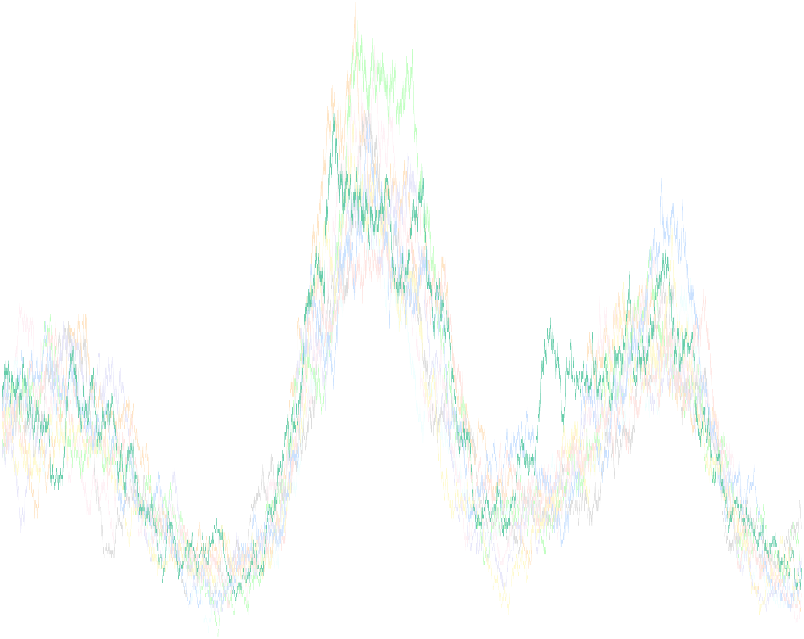
\includegraphics[height=10cm, width=20cm]{images/titlepic.pdf} }
\title{Spatial Epidemics Dynamics: Synchronization}
\subtitle{Mathematics 4MB3/6MB3\\Mathematical Biology}
\date{\today}
\author{Model Students: Nicole Dumont, Melody Fong, Carolina Weishaar}
\IfFileExists{upquote.sty}{\usepackage{upquote}}{}
\begin{document}
%\SweaveOpts{concordance=TRUE}
  \maketitle
  
%%% Table of Contents
\begin{frame}{Table of Contents}
  \setbeamertemplate{section in toc}[sections numbered]
  \tableofcontents[hideallsubsections]
\end{frame}

%%% Introduction to the topic with examples
\section{Introduction}
  \begin{frame}{\textit{Ailuropoda melanoleuca}}
    \centering \includegraphics[width=.90\linewidth]{images/{"Panda0"}.pdf}
  \end{frame}

  \begin{frame}{Current Habitat}
    \centering \includegraphics[width=.90\linewidth]{images/{"MapPanda"}.pdf}
  \end{frame}

  \begin{frame}{Synchronization}
    \begin{itemize}
      \item First observed in nonlinear systems by Christian Huygens in 1665.
      %\item \bf{Definition}:
    \end{itemize}
  \end{frame}
  
  \begin{frame}{Weekly measles case reports for Birmingham, Newcastle,\\ Cambridge and Norwich between 1944 and 1958}
    \centering \includegraphics[width=.90\linewidth]{images/{"fig1"}.pdf}
  \end{frame}
  
  \begin{frame}{Wavelet phase analysis of weekly measles reports for\\ Cambridge, Norwich and London between 1994 and 1996}
    \centering \includegraphics[width=.90\linewidth]{images/{"Travelling waves and spatial hierarchies in measles epidemics - Grenfell"}.pdf}
  \end{frame}
  
  \begin{frame}{The effects of mobility on the persistence of a population}
    \centering \includegraphics[width=.90\linewidth]{images/{"fig7"}.pdf}
  \end{frame}
  
%%%% Methods Used in Project
\section{Methods}
  \begin{frame}{Forced SIR Model for a Single Patch}
    \begin{center}
    
    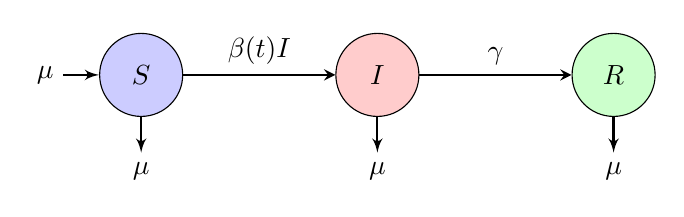
\begin{tikzpicture}[node distance=3cm,auto,>=latex',every node/.append style={align=center}]
      \node [int, pin={[pinstyleto]left:$\mu$}, pin={[pinstyleout]below:$\mu$}] (a)              {$S$};
      \node [int2, pin={[pinstyleout]below:$\mu$}] (b) [right of=a] {$I$};
      \node [int3, pin={[pinstyleout]below:$\mu$}] (c) [right of=b] {$R$};
    
      \draw [arrow] (a) -- node[anchor=south] {$ \beta(t) I $} (b);
      \draw [arrow] (b) -- node[anchor=south] {$\gamma$} (c);
    \end{tikzpicture}
    \begin{align*}
      \frac{dS}{dt} &= \mu -\textcolor{orange}{\beta(t)} S I -\mu S \\ 
      \frac{dI}{dt} &= \textcolor{orange}{\beta(t)} S I -\gamma I - \mu I \\
      \frac{dR}{dt} &= \gamma I -\mu R
    \end{align*}

    \begin{alertblock}{
    \begin{align*}
      \beta(t) &= \left < \beta \right > (1+\alpha \cos(2\pi t)) \\
      \left < \beta \right > &= \mathcal{R}_0 (\mu + \gamma)
    \end{align*}
    }\end{alertblock}
  
    \end{center}
  \end{frame}
  
  \begin{frame}{Metapatch SIR Model}
    \begin{center}
    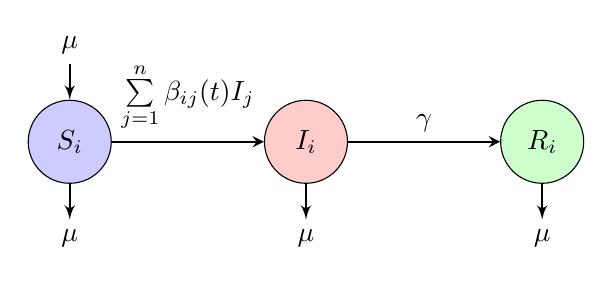
\begin{tikzpicture}[node distance=3cm,auto,>=latex',every node/.append style={align=center}]
      \node [int, pin={[pinstyleto]above:$\mu$}, pin={[pinstyleout]below:$\mu$}] (a)   {$S_i$};
      \node [int2, pin={[pinstyleout]below:$\mu$}] (b) [right of=a] {$I_i$};
      \node [int3, pin={[pinstyleout]below:$\mu$}] (c) [right of=b] {$R_i$};
    
     \draw [arrow] (a) -- node[anchor=south] {$ \sum\limits_{j=1}^{n}\beta_{ij}(t) I_j $} (b);
     \draw [arrow] (b) -- node[anchor=south] {$\gamma$} (c);
    \end{tikzpicture}
    \begin{align*}
      \frac{dS_i}{dt} &= \mu - S_i\sum\limits_{j=1}^{n}\beta_{ij}(t) I_j -\mu S_i \\ 
      \frac{dI_i}{dt} &= S_i\sum\limits_{j=1}^{n}\beta_{ij}(t) I_j -\gamma I_i - \mu I_i \\
      \frac{dR_i}{dt} &= \gamma I_i -\mu R_i
    \end{align*}
    \end{center}
  \end{frame}
   
  \begin{frame}{Beta Matrix}
    \begin{equation*}
      \beta(t) = \left < \beta \right > (1+\alpha \cos(2\pi t))M
    \end{equation*}
    \metroset{block=fill}
    \begin{alertblock}{Equal Coupling Matrix}
      \[
      M =
      \begin{bmatrix}
      1-m & \frac{m}{n-1} & \frac{m}{n-1} & \frac{m}{n-1} & \dots \\
      \frac{m}{n-1} & 1-m & \frac{m}{n-1} & \frac{m}{n-1}  \\
      \frac{m}{n-1} & \frac{m}{n-1} & 1-m &  \\
      \vdots &  &  & \ddots 
      \end{bmatrix}
      \]
    \end{alertblock}
  \end{frame}
  
  \begin{frame}{Beta Matrix}
    \begin{equation*}
      \beta(t) = \left < \beta \right > (1+\alpha \cos(2\pi t))M
    \end{equation*}
    \metroset{block=fill}
    \begin{alertblock}{Nearest Neighbour Matrix}
      \[
      M =
      \begin{bmatrix}
      1-m & \frac{m}{2} & 0 & 0 & \dots & \frac{m}{2} \\
      \frac{m}{2} & 1-m & \frac{m}{2} & 0 & & \vdots \\
      0 & \frac{m}{2} & 1-m &  \\
      0 & 0 & & \ddots \\
      \vdots & & & & \ddots & \frac{m}{2} \\
      \frac{m}{2} &  & & \dots & \frac{m}{2} & 1-m \ 
      \end{bmatrix}
      \]
    \end{alertblock}
  \end{frame}
  
  \begin{frame}{Modelling Stochasticity}
  The effects of stochasticity are crucial in this model
  \pause 
  \metroset{block=fill}
      \begin{alertblock}{Exact Simulation: Gillespie Algorthim}
      \begin{itemize}
        \item Get waiting time by sample from an exponential distribution with parameter equal to the total transition rate
        \item Randomly select which transition occurred with probability given by its transition rate relative to the total rate
        \item Unfeasible for large populations
        \end{itemize}
      \end{alertblock}
  \end{frame}
  
  \begin{frame}{Modelling Stochasticity}
  \metroset{block=fill}
      \begin{alertblock}{Approximate Simulation: Adaptive Tau Algorthim}
      \begin{itemize}
      \item The \texttt{adaptivetau} package
        \item Find time periods where transition rates are approximately constant
        \item Skip this time and use a Possion distribution to approximate which transitions occured 
        \end{itemize}
      \end{alertblock}
  \end{frame}
  
%%% Results of simulations and models  
\section{Results}
  
  \begin{frame}{Bifurcation Diagram}
   Single Patch SIR model with sinusoidal seasonal forcing
   \centering 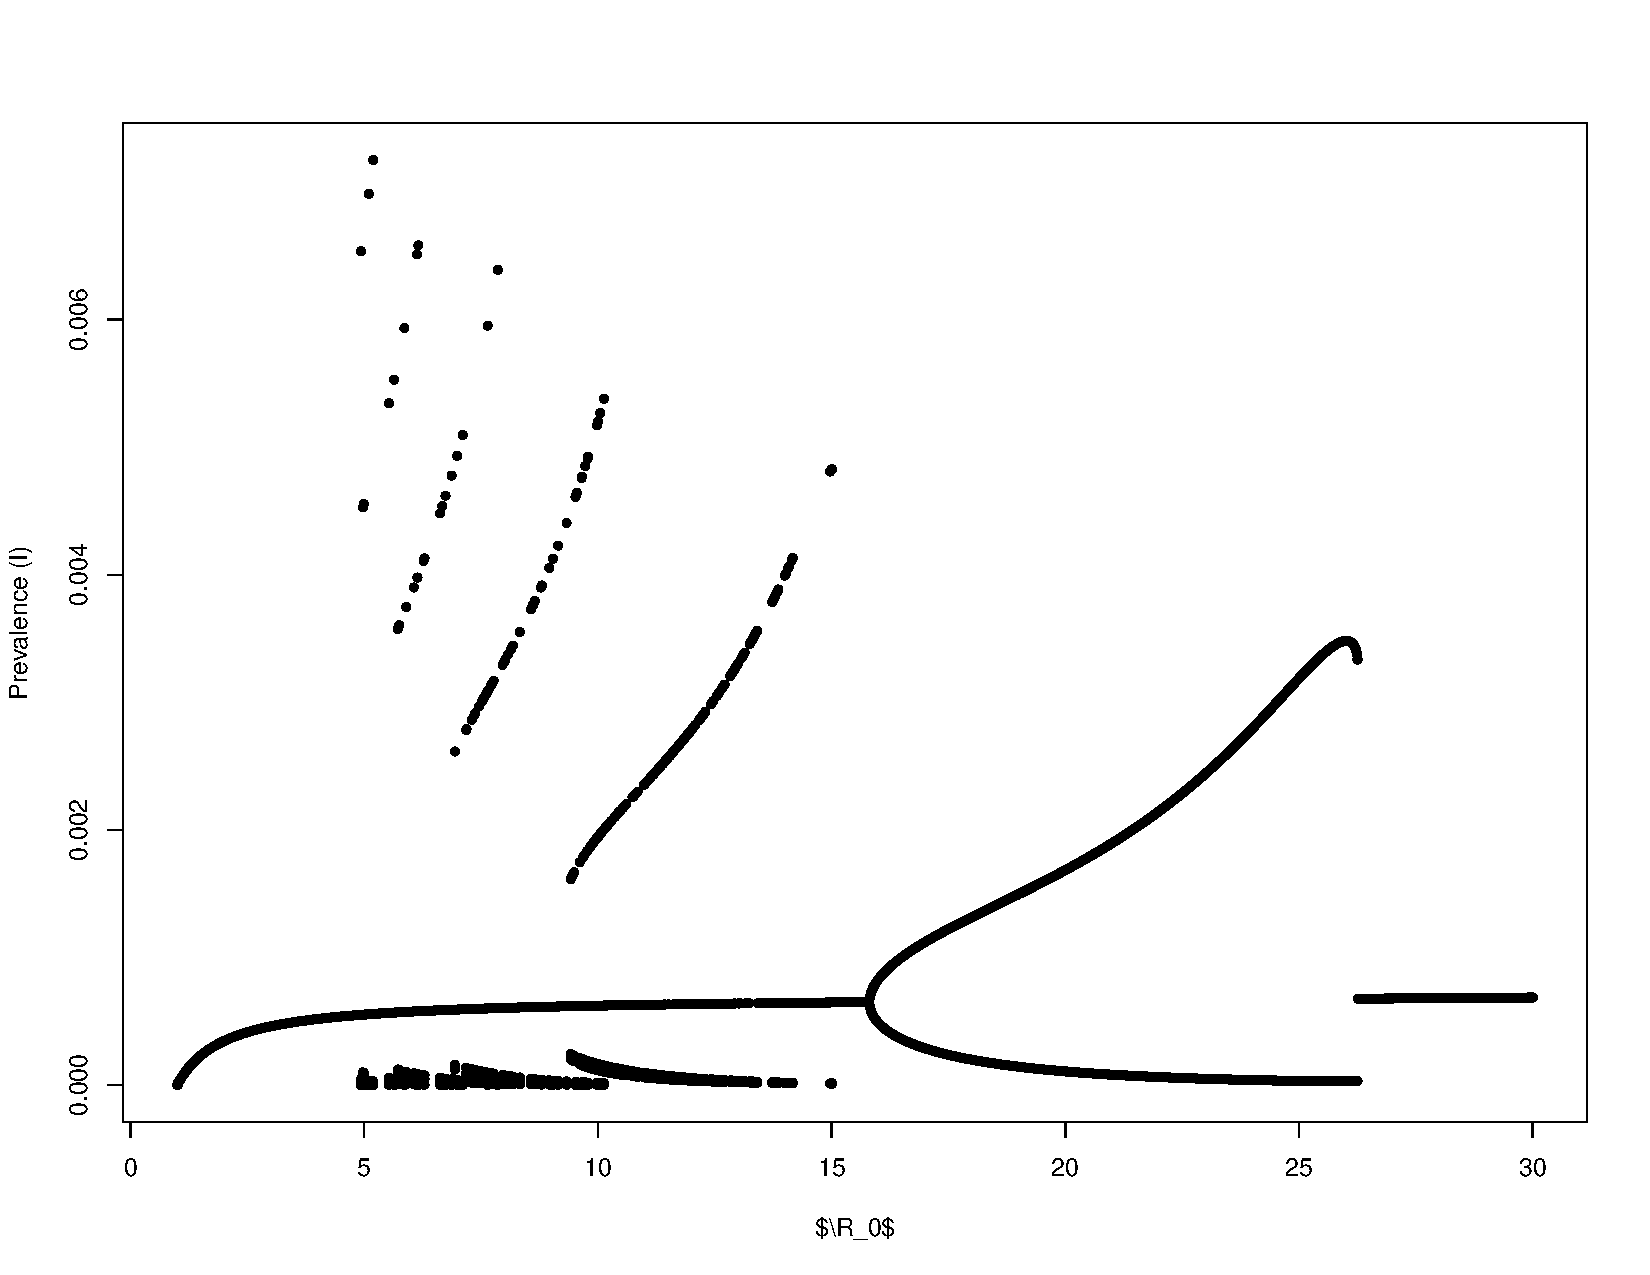
\includegraphics[width=0.7\linewidth]{{images/bifurcation}.pdf}
  \end{frame}
   
  \begin{frame}{Period Diagram}
   Period of the oscillations
   \centering 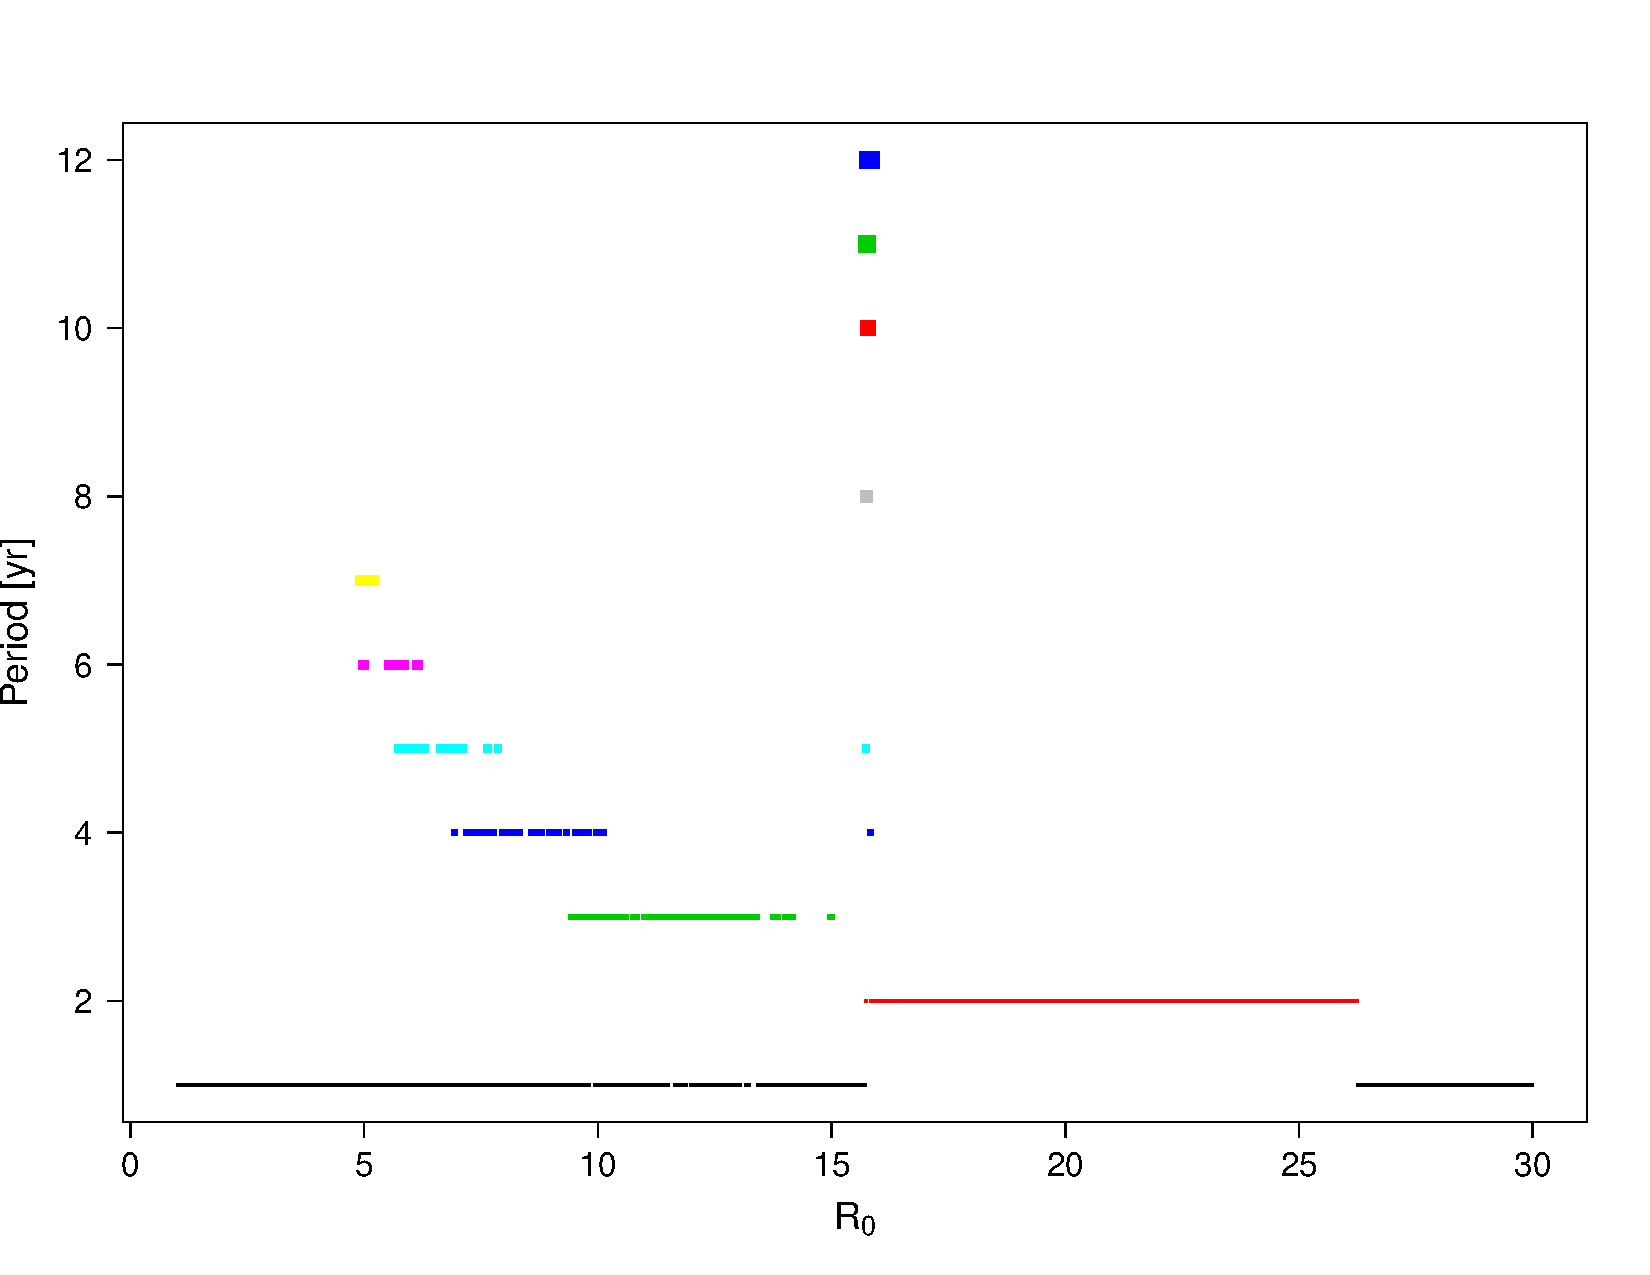
\includegraphics[width=0.7\linewidth]{{images/period}.pdf}
  \end{frame}

  \begin{frame}{Deterministic Model}
   Equal Coupling, $\mathcal{R}_0=17$, $m=0.2$
   \centering 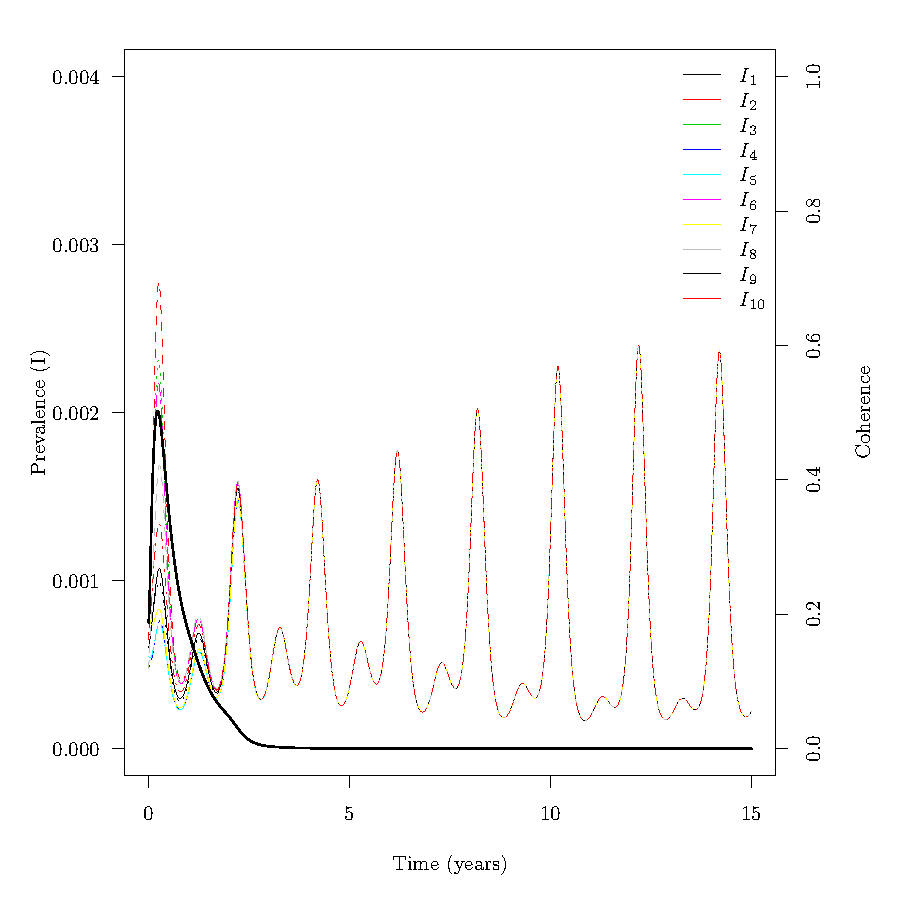
\includegraphics[width=0.7\linewidth]{{images/detECR017m0.2}.pdf}
  \end{frame}
   
  \begin{frame}{Deterministic Model: EC vs NN}
   \begin{centering}
   $\mathcal{R}_0=17$, $m=0.2$
     \begin{columns}[T,onlytextwidth]
     
      \begin{column}{0.5\textwidth}
      \scalebox{0.8}{\parbox{.5\linewidth}{%
       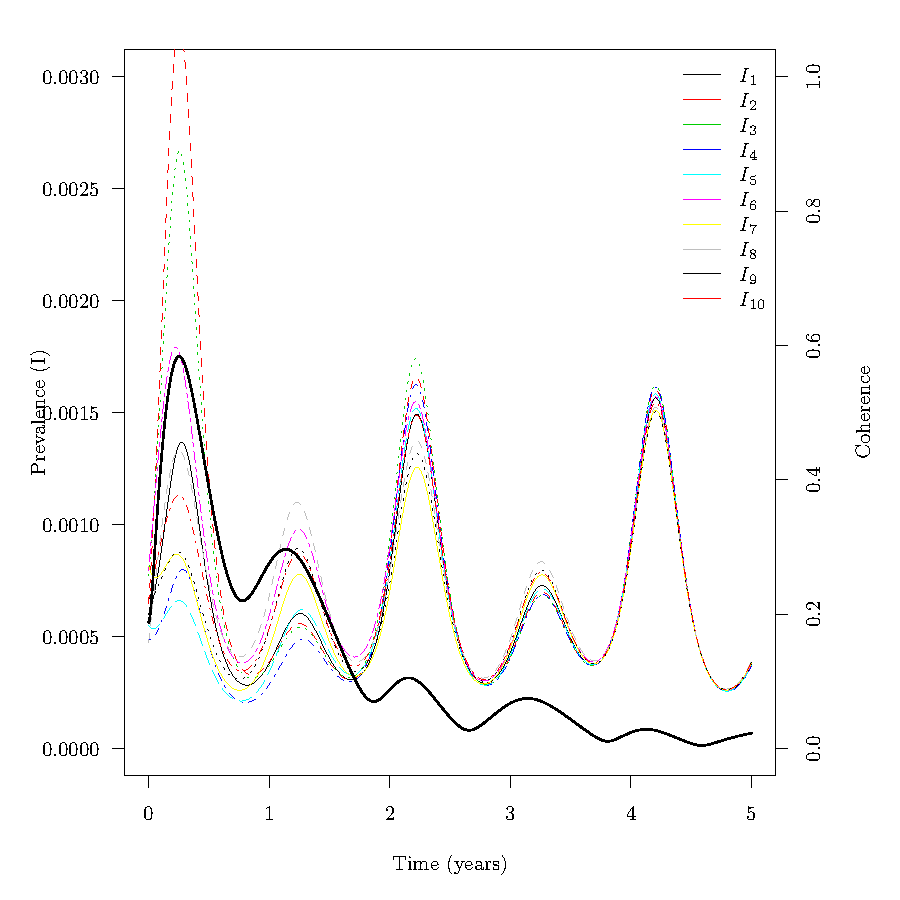
\includegraphics[width=2.2\linewidth]{{images/detNNR017m0.2s}.pdf} \\
       \metroset{block=fill}
      \begin{block}{Nearest Neighbour Coupling}
      \end{block}
      }}
     \end{column}
    \begin{column}{0.5\textwidth}
    \scalebox{0.8}{\parbox{.5\linewidth}{%
       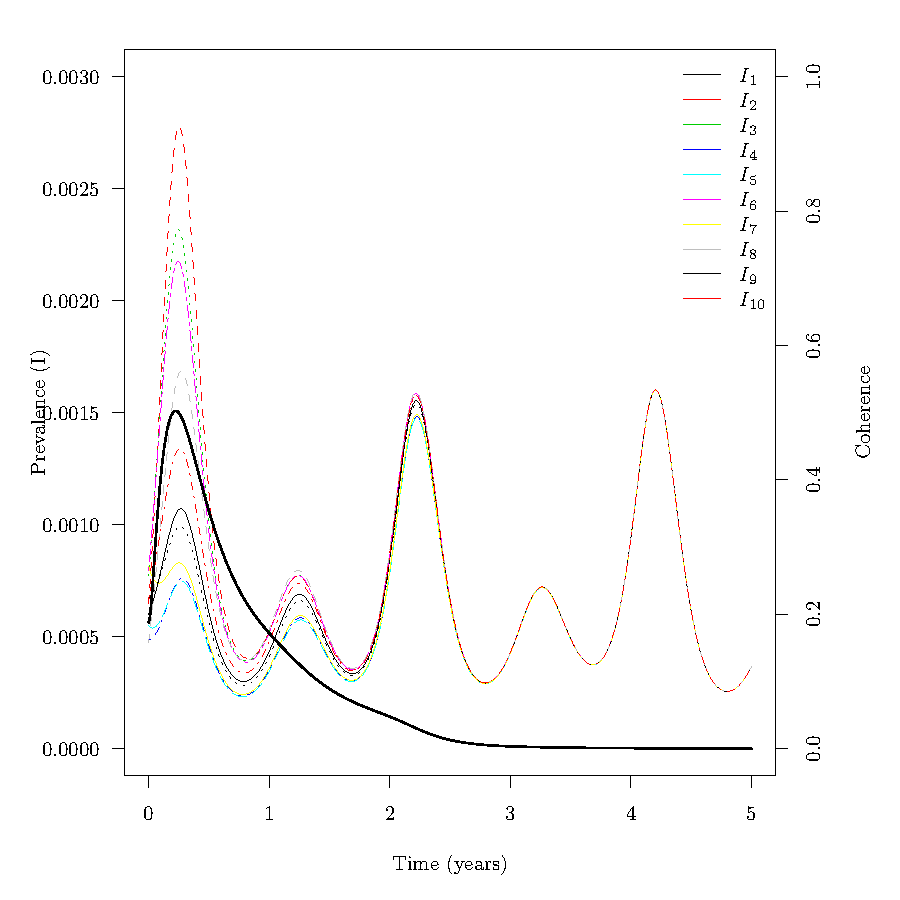
\includegraphics[width=2.2\linewidth]{{images/detECR017m0.2s}.pdf} \\
       \metroset{block=fill}
       \begin{block}{Equal Coupling}
      \end{block}
      }}
    \end{column}
    \end{columns}
    \end{centering}
  \end{frame}
   
  \begin{frame}{Deterministic Model}
    \begin{centering}
     Nearest Neighbour Coupling, $\mathcal{R}_0=17$, $m=0.01$
     \begin{columns}[T,onlytextwidth]
      \begin{column}{0.5\textwidth}
      \scalebox{0.8}{\parbox{.5\linewidth}{%
       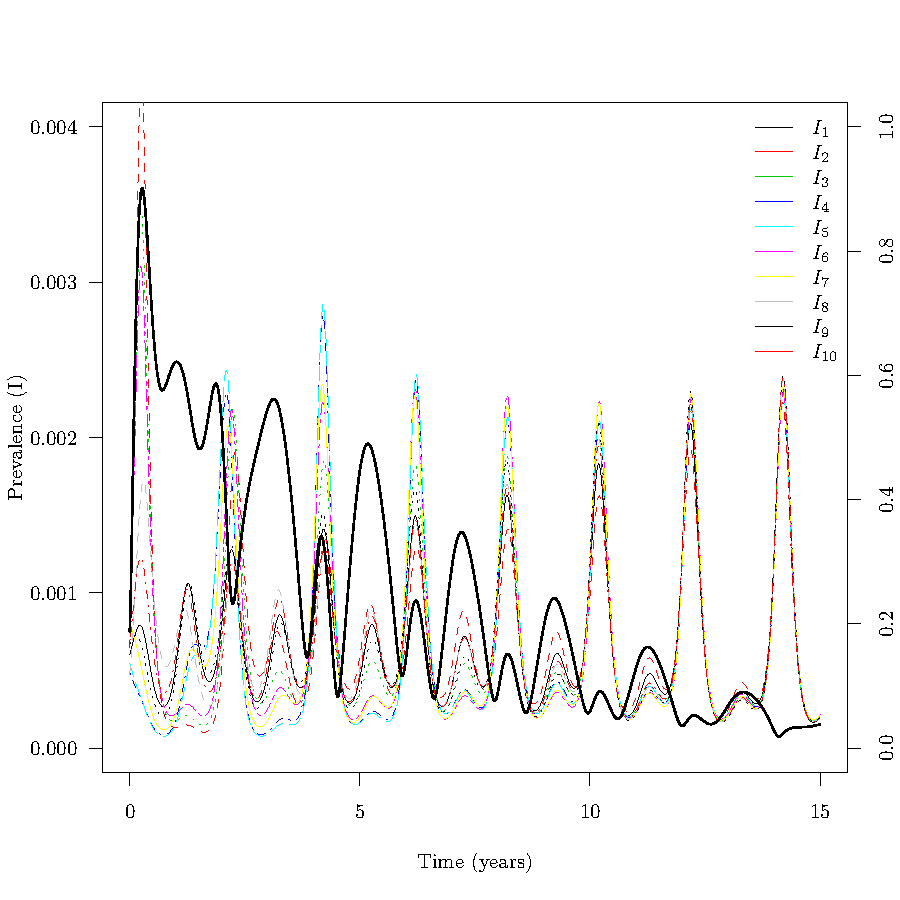
\includegraphics[width=2.2\linewidth]{{images/detNNR017m0.01}.pdf} \\
        
      \metroset{block=fill}
      \begin{alertblock}{Initial Conditions}
        Within 30\% percent of endemic equilibrium
      \end{alertblock}
      }}
     \end{column}
    \begin{column}{0.5\textwidth}
    \scalebox{0.8}{\parbox{.5\linewidth}{%
       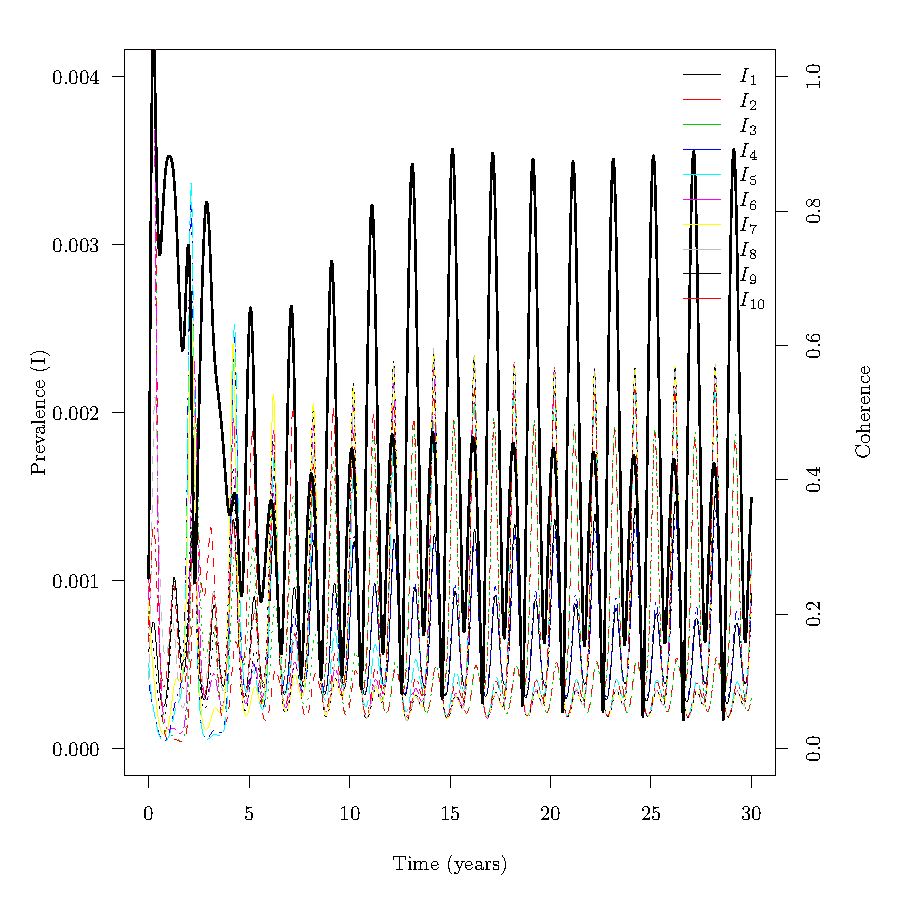
\includegraphics[width=2.2\linewidth]{{images/detNNR017m0.01wider}.pdf} \\
       \metroset{block=fill}
      \begin{alertblock}{Initial Conditions}
        Within 40\% percent of endemic equilibrium
      \end{alertblock}
      }}
    \end{column}
    \end{columns}
    \end{centering}
  \end{frame}
   
  \begin{frame}{Deterministic Model}
   \begin{centering}
     Nearest Neighbour Coupling, $m=0.2$
     \begin{columns}[T,onlytextwidth]
      \begin{column}{0.5\textwidth}
      \scalebox{0.8}{\parbox{.5\linewidth}{%
       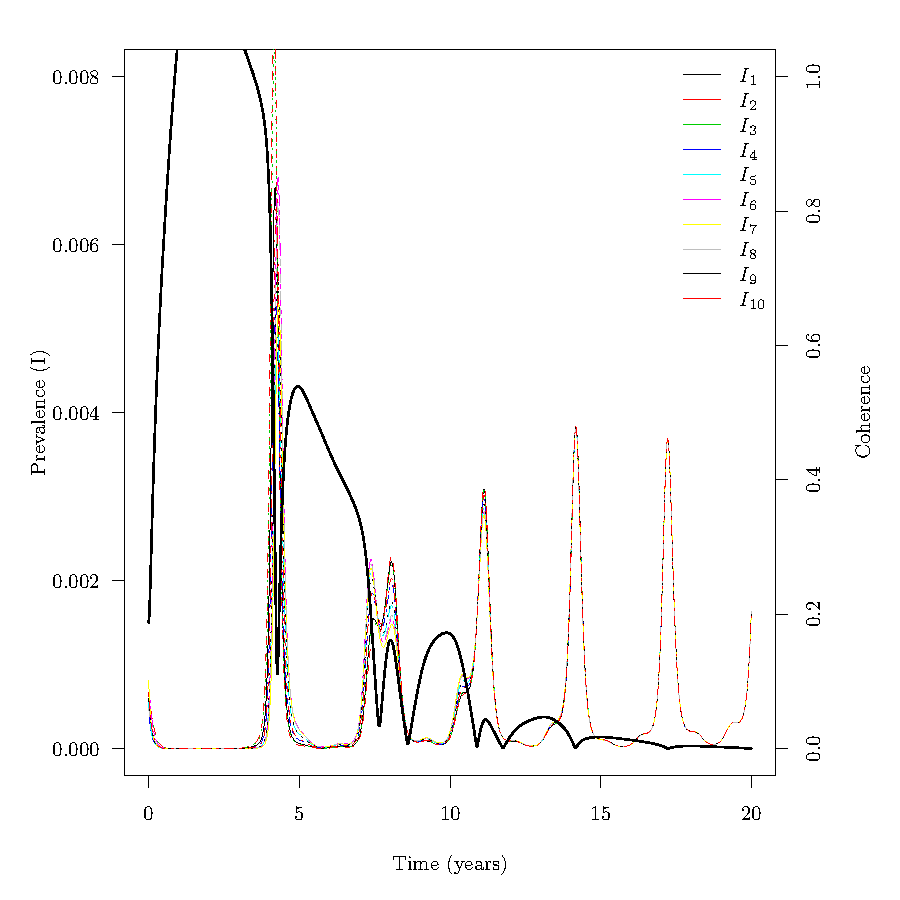
\includegraphics[width=2.2\linewidth]{{images/detNNR010m0.2}.pdf} \\
       \metroset{block=fill} \begin{block}{$\mathcal{R}_0=10$}
      \end{block}
      
      }}
     \end{column}
    \begin{column}{0.5\textwidth}
    \scalebox{0.8}{\parbox{.5\linewidth}{%
       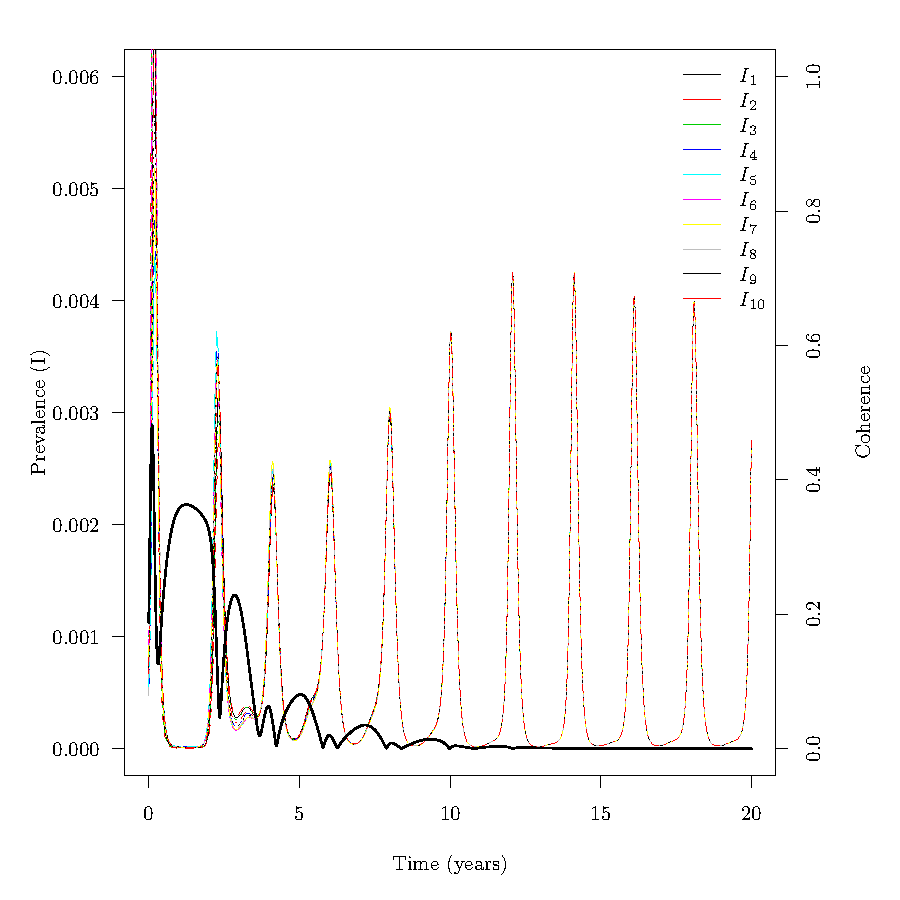
\includegraphics[width=2.2\linewidth]{{images/detNNR025m0.2}.pdf} \\
       \metroset{block=fill} \begin{block}{$\mathcal{R}_0=25$}
      \end{block}
       
      }}
    \end{column}
    \end{columns}
    \end{centering}
  \end{frame}
   
  \begin{frame}{Stochastic: Gillespie Model}
   Equal Coupling, Population of 3000, $\mathcal{R}_0=17$, $m=0.2$
   \centering 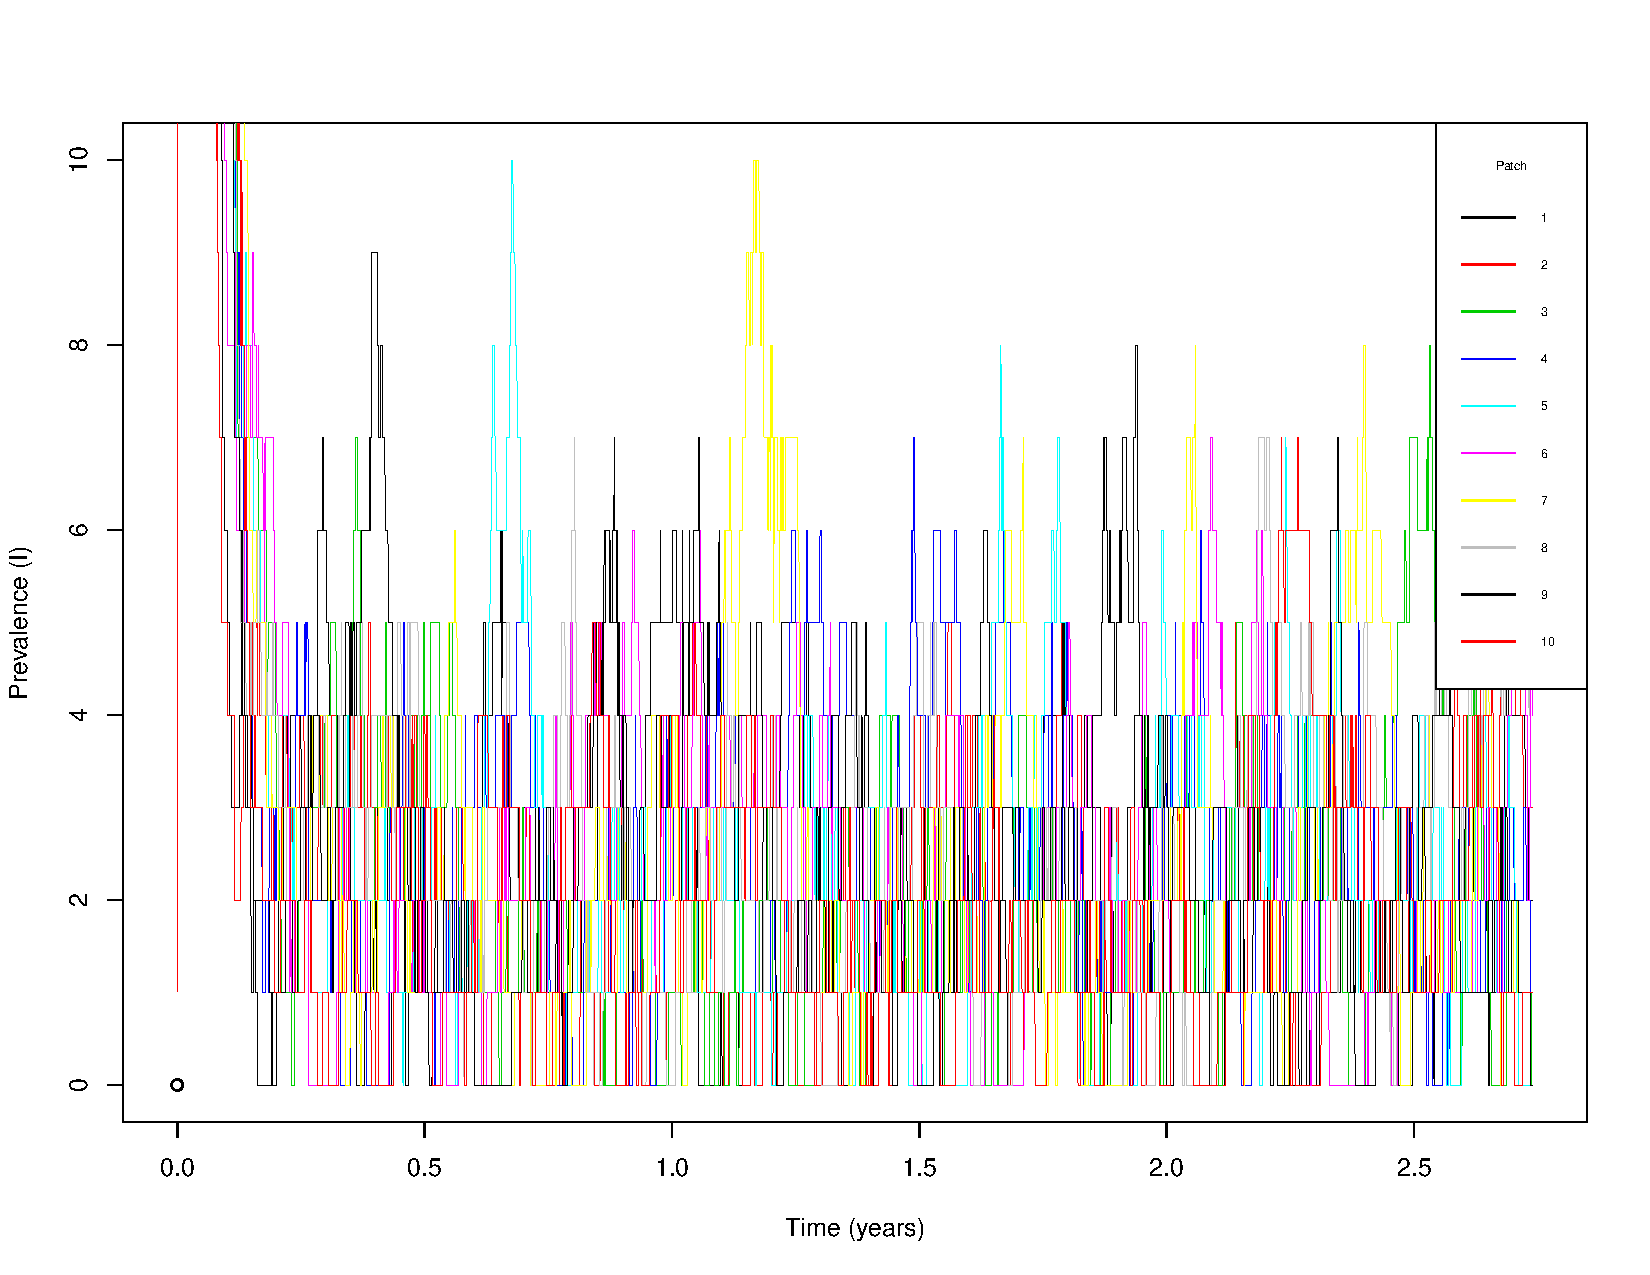
\includegraphics[width=0.7\linewidth]{{images/GillECR017m0.2small}.pdf}
   \end{frame}
   
   \begin{frame}{Stochastic: Gillespie Model}
   Equal Coupling, Population of 100,000, $\mathcal{R}_0=17$, $m=0.2$ 
   \centering 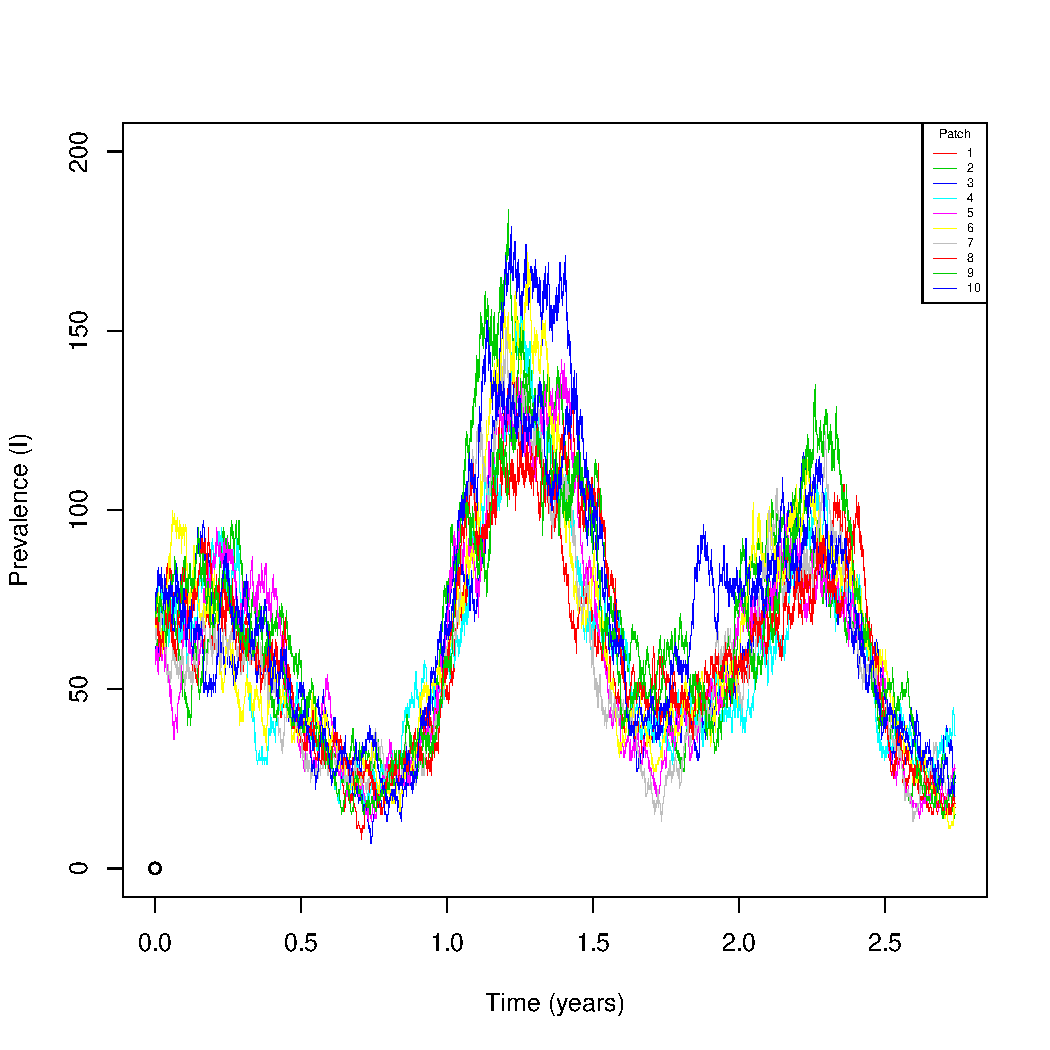
\includegraphics[width=0.6\linewidth]{{images/GillECR017m0.2}.pdf}\\
   \centering \alert{3 hour run time!}
   \end{frame}
   
     \begin{frame}{Adaptive Tau Algorthim}
   
  \end{frame}
   
  \begin{frame}{Stochastic: Adaptive Tau Algorthim}
    Equal Coupling, Population of 500,000, $\mathcal{R}_0=17$, $m=0.2$
    \centering 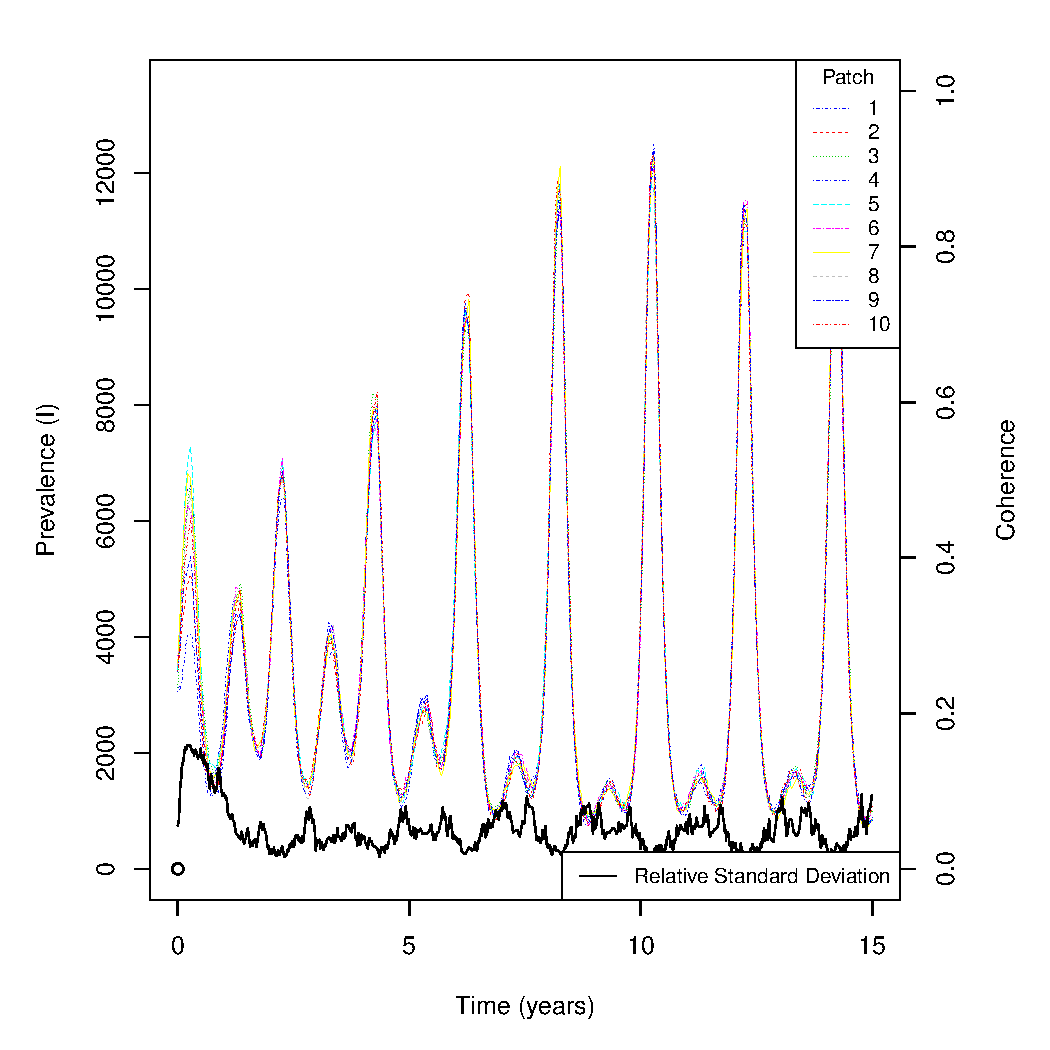
\includegraphics[width=0.7\linewidth]{{images/adaptauECR017m0.2}.pdf}
  \end{frame}
   
  \begin{frame}{Stochastic: Adaptive Tau Algorthim}
    Equal Coupling, Population of 500,000, $\mathcal{R}_0=17$, $m=0.01$
    \centering 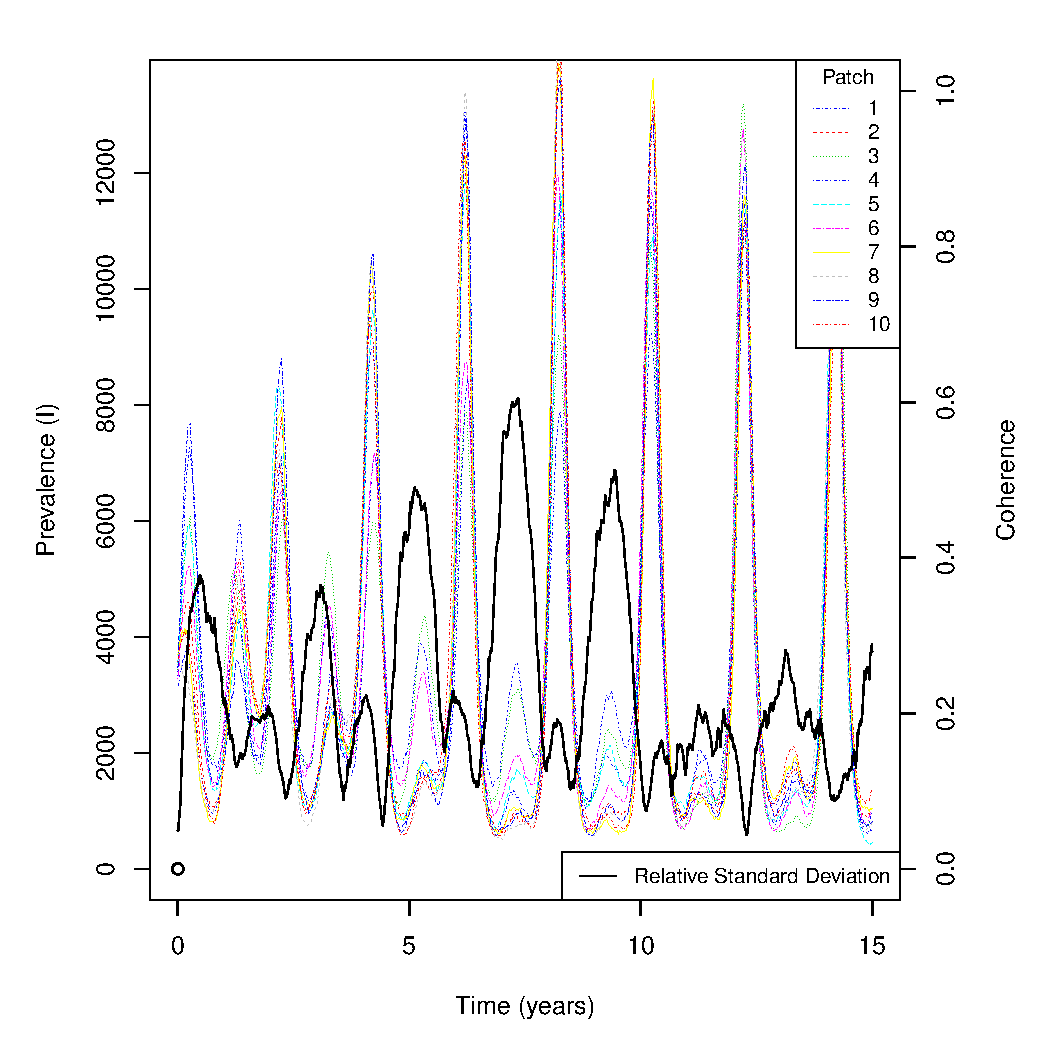
\includegraphics[width=0.7\linewidth]{{images/adaptauECR017m0.01}.pdf}
  \end{frame}
   
  \begin{frame}{Stochastic: Adaptive Tau Algorthim}
    Equal Coupling, Population of 500,000, $\mathcal{R}_0=25$, $m=0.2$
    \centering 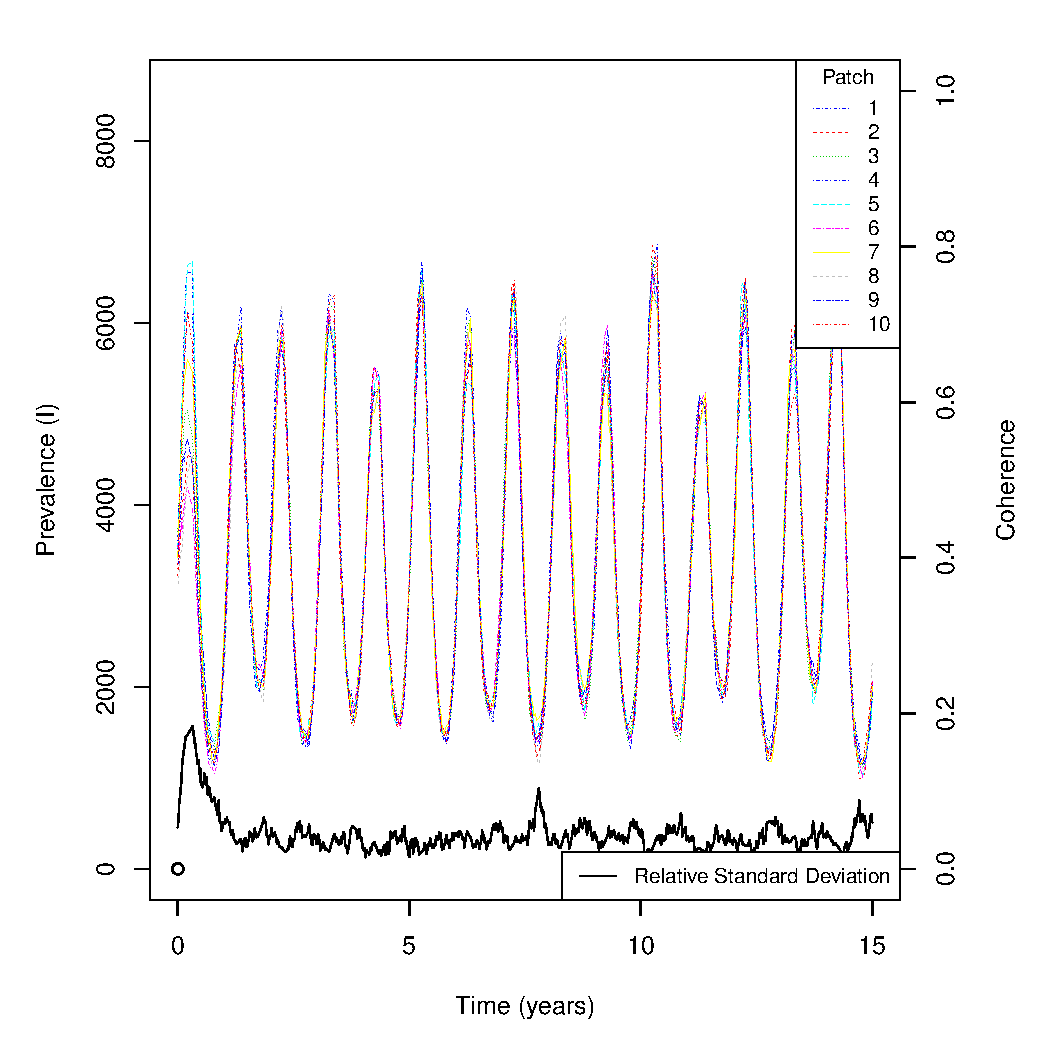
\includegraphics[width=0.7\linewidth]{{images/adaptauECR025m0.2}.pdf}
  \end{frame}
   
  \begin{frame}{Coherence dependence on Parameters}
    Equal Coupling, Population of 250,000,\\ $80 \times 80$ grid, 5 simulations per grid point
    \centering 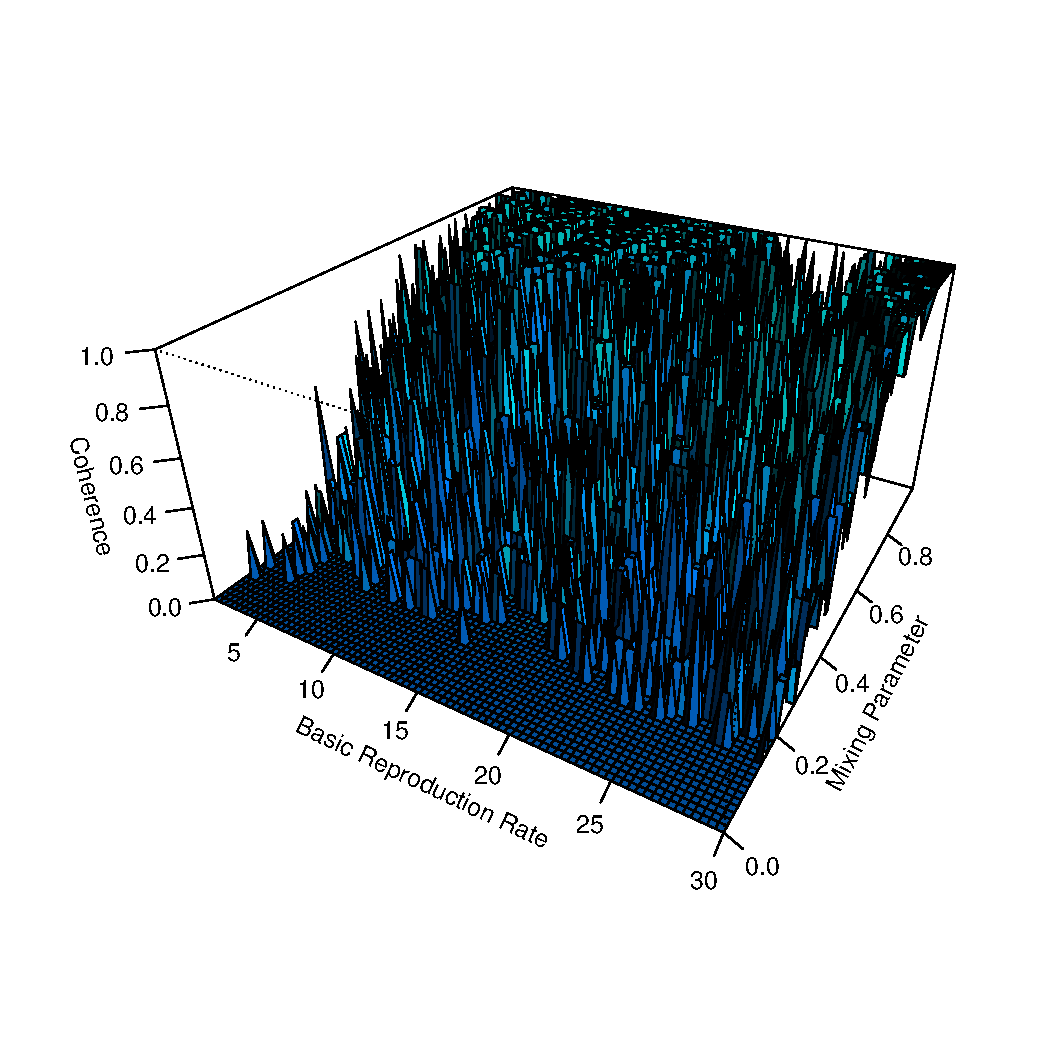
\includegraphics[width=0.7\linewidth]{{images/Adaptau3DEC}.pdf}
  \end{frame}
   
  \begin{frame}{Coherence dependence on Parameters}
    Nearest Neighbour Coupling, Population of 250,000,\\ $80 \times 80$ grid, 5 simulations per grid point
    \centering 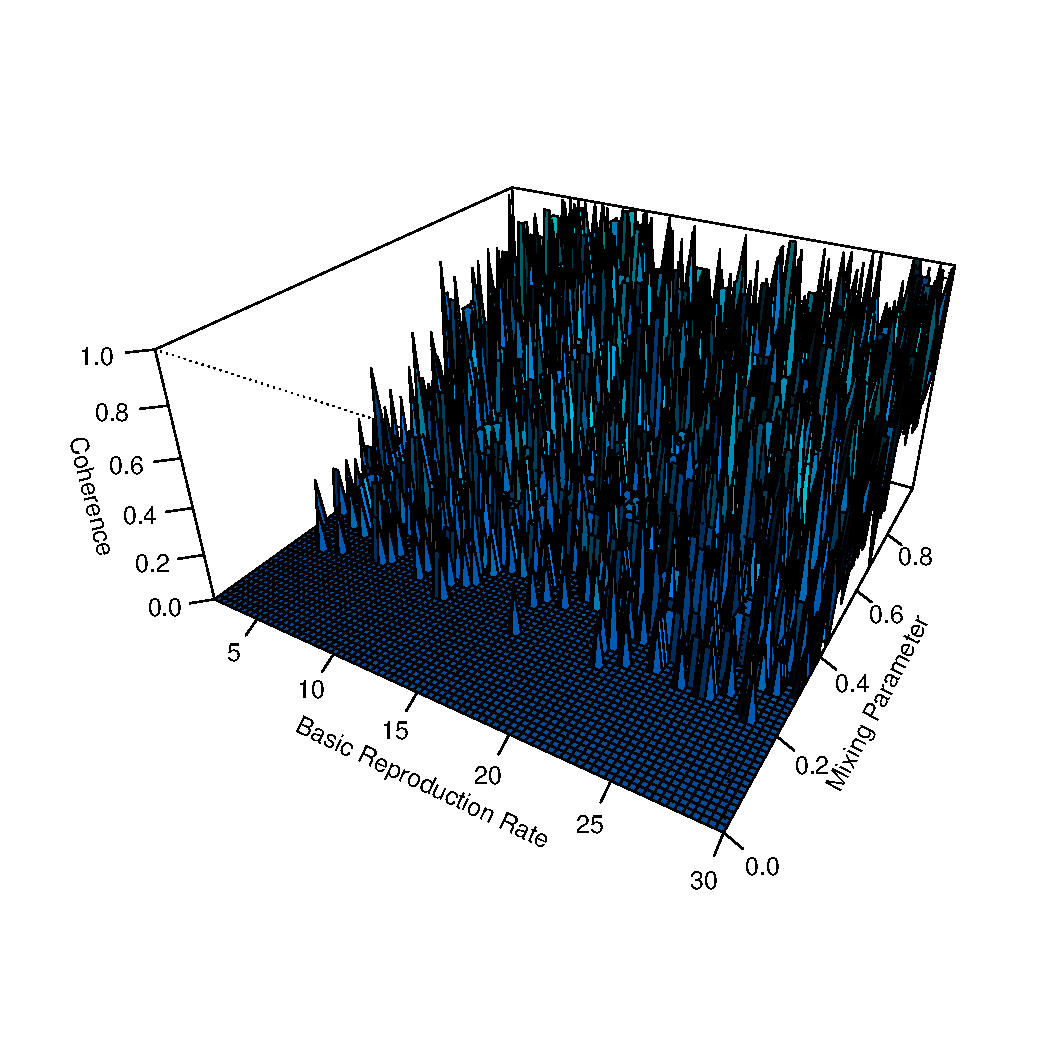
\includegraphics[width=0.7\linewidth]{{images/Adaptau3DNN}.pdf}
  \end{frame}
   
  \begin{frame}{Coherence dependence on Parameters}
    Nearest Neighbour Coupling, Population of 250,000, 5 simulations per grid point \\
    \centering 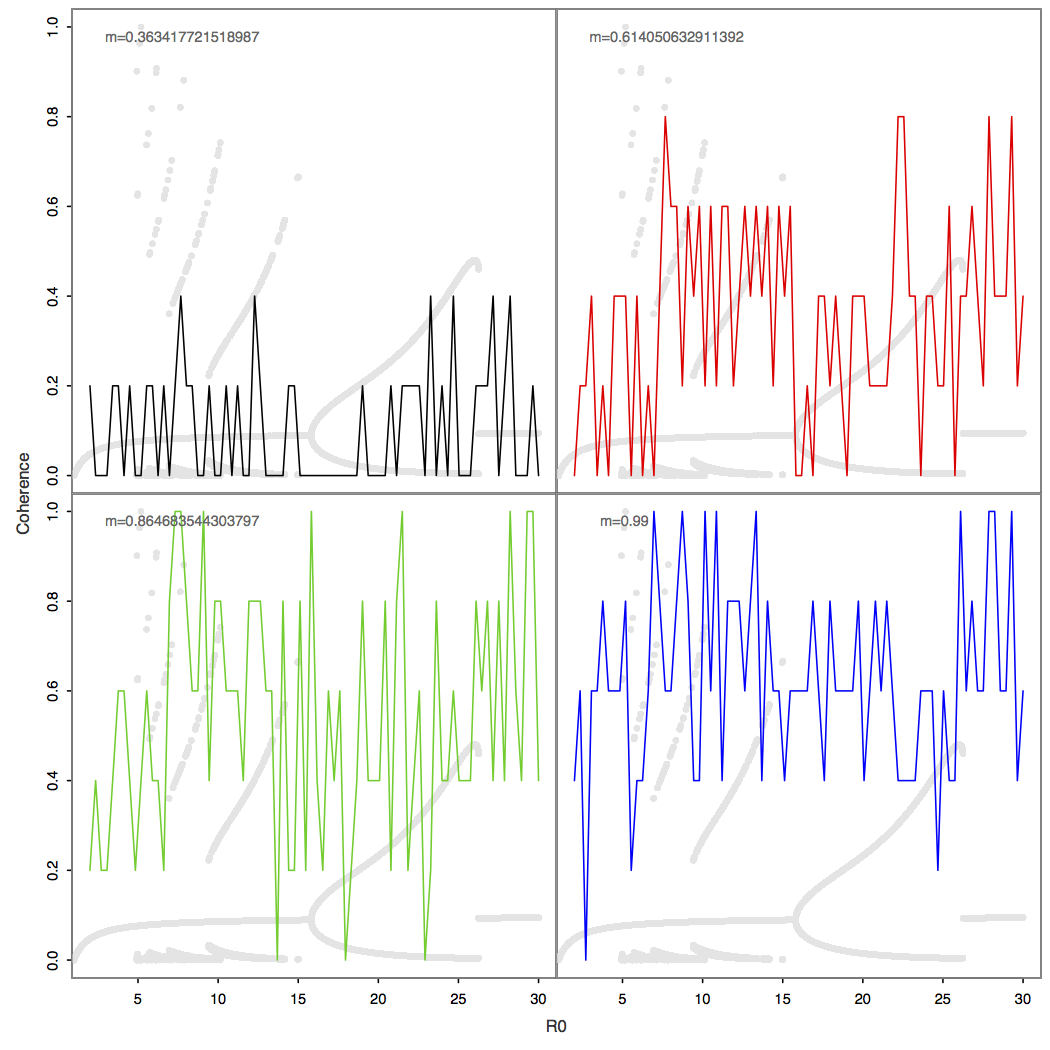
\includegraphics[height=6cm,width=0.7\linewidth]{{images/FourPanelNN}.png}
  \end{frame}
 
%%% Conclusions  
\section{Conclusion}
  \begin{frame}
    \begin{itemize}
      \item Importance of synchronization
      \pause\item Coherence dependence on parameters
      \pause\item Further study
    \end{itemize}
  \end{frame}
   
%% Questions slide  
\begin{frame}[standout]
  Questions?
\end{frame}

\appendix
\begin{frame}[allowframebreaks]{References}
  \nocite{*}
  \bibliographystyle{abbrv}
  \bibliography{ModelStudents.bib}
\end{frame}


   
\end{document}
